\setchapterpreamble[u]{\margintoc} 
\chapter{Analyser et valider les performances d'un système} 
\section{Réaliser une analyse structurelle, flux, effort} 
\graphicspath{{\repStyle/png/}{../SYS-01/SYS-01_ChaineFonctionnelle/58_Oz440/images/}} 
\normaltrue \difficilefalse \tdifficilefalse
\correctiontrue

%\UPSTIidClasse{11} % 11 sup, 12 spé
%\newcommand{\UPSTIidClasse}{12}
% CCP MP 2016
\exer{Robot de maraîchage Oz 440 $\star$ \label{SYS:01:58}}
\setcounter{question}{0}
\marginnote[5cm]{\xpComp{SYS}{01}}
\index{Compétence SYS-01}
\index{Robot de maraîchage Oz 440 }
\index{Associer les fonctions aux constituants.}

\ifcorrection
\else
\marginnote{\textbf{Pas de corrigé pour cet exercice.}}
\fi

\ifprof
\else

Le robot de maraîchage Oz 440 développé par la société Naïo Technologies est un outil autonome
agricole, alliant robustesse et écologie, capable d’assister les maraîchers dans les tâches les plus
pénibles comme le transport de charges lors des récoltes et le désherbage mécanique à l’aide d’un
outil de binage.


\begin{figure}[H]
\centering
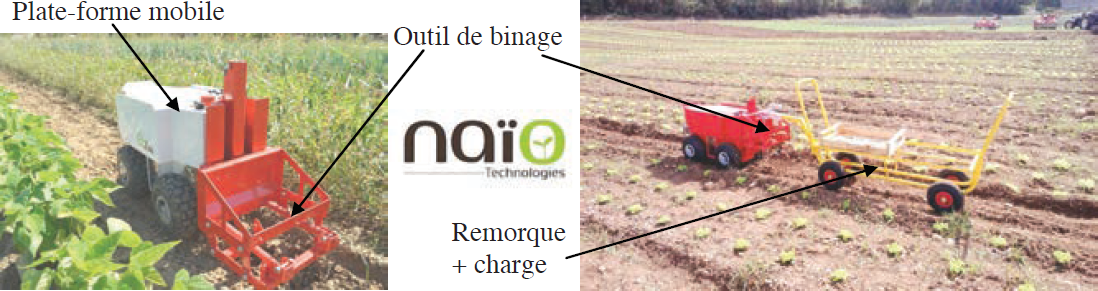
\includegraphics[width=\linewidth]{58_01}
%\caption{Amplificateur de charge à plusieurs canaux KISTLER. \label{fig_50_01}}
\end{figure}


Ce robot est constitué d’une plate-forme mobile électrique à 4 roues motrices sur laquelle sont
fixés divers outils et capteurs. La figure 1 donne la structure du robot sous la forme d’un
diagramme de définition de blocs (BDD) avec les propriétés principales de chaque constituant,
utiles pour la résolution du problème.

\begin{figure}[H]
\centering
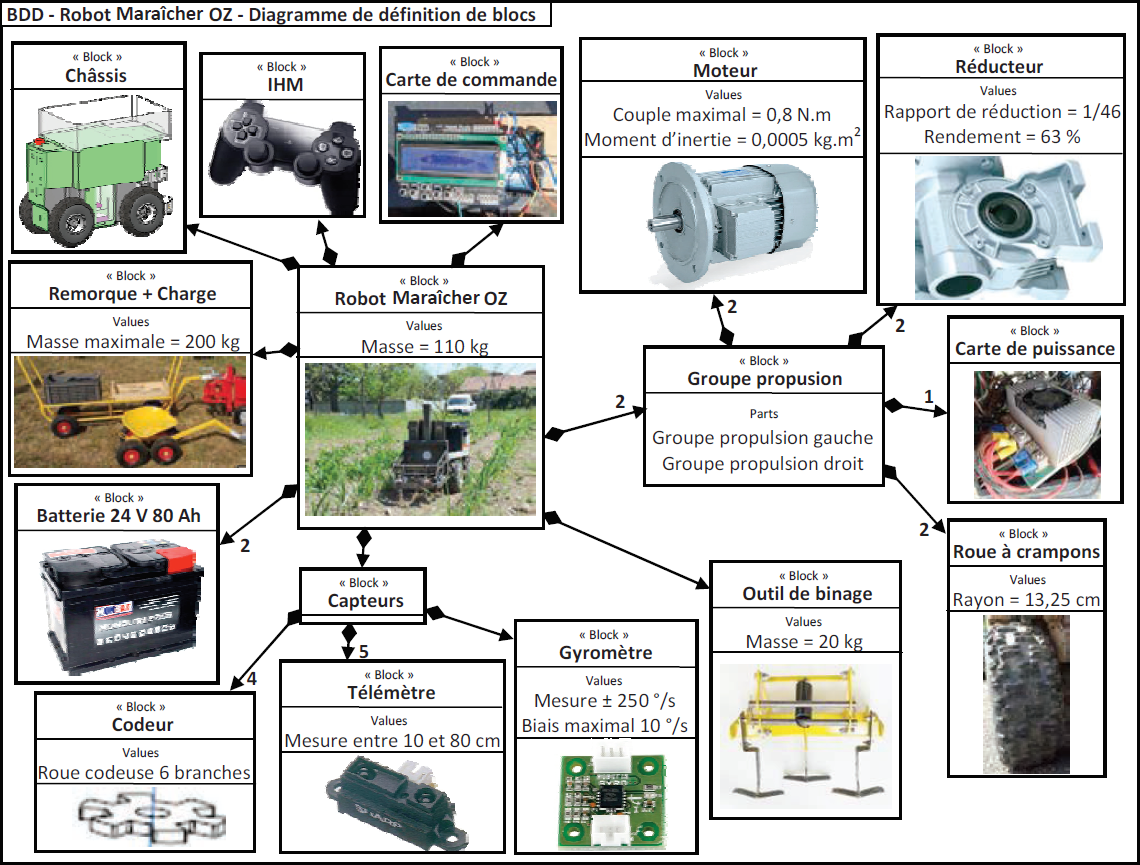
\includegraphics[width=\linewidth]{58_02}
%\caption{Amplificateur de charge à plusieurs canaux KISTLER. \label{fig_50_01}}
\end{figure}


Ce robot de petite taille évolue directement entre les rangées de cultures pour un travail de
précision. Il peut, par exemple, désherber et aussi suivre des personnes lors de la récolte tout en
transportant des charges. Bien plus petit qu’un tracteur classique, il ne casse pas la structure
naturelle du sol et évite ainsi le phénomène de compaction des sols provoqué habituellement par les
tracteurs ou le piétinement de l’homme. Il roule lentement et passe au plus près des cultures sans
risquer de les abîmer. Selon le vieil adage « un binage vaut deux arrosages », le fait de pouvoir
utiliser ce robot régulièrement, sans perte de temps, permet de toujours avoir un sol parfaitement
biné et ainsi de diminuer les effets d’évaporation de l’eau.
\fi

\question{À l’aide du diagramme de définition de blocs disponible, réaliser le diagramme correspondant à la chaîne fonctionnelle de l’ensemble
groupe propulsion droit du robot.}
\ifprof

\begin{figure}[H]
\centering
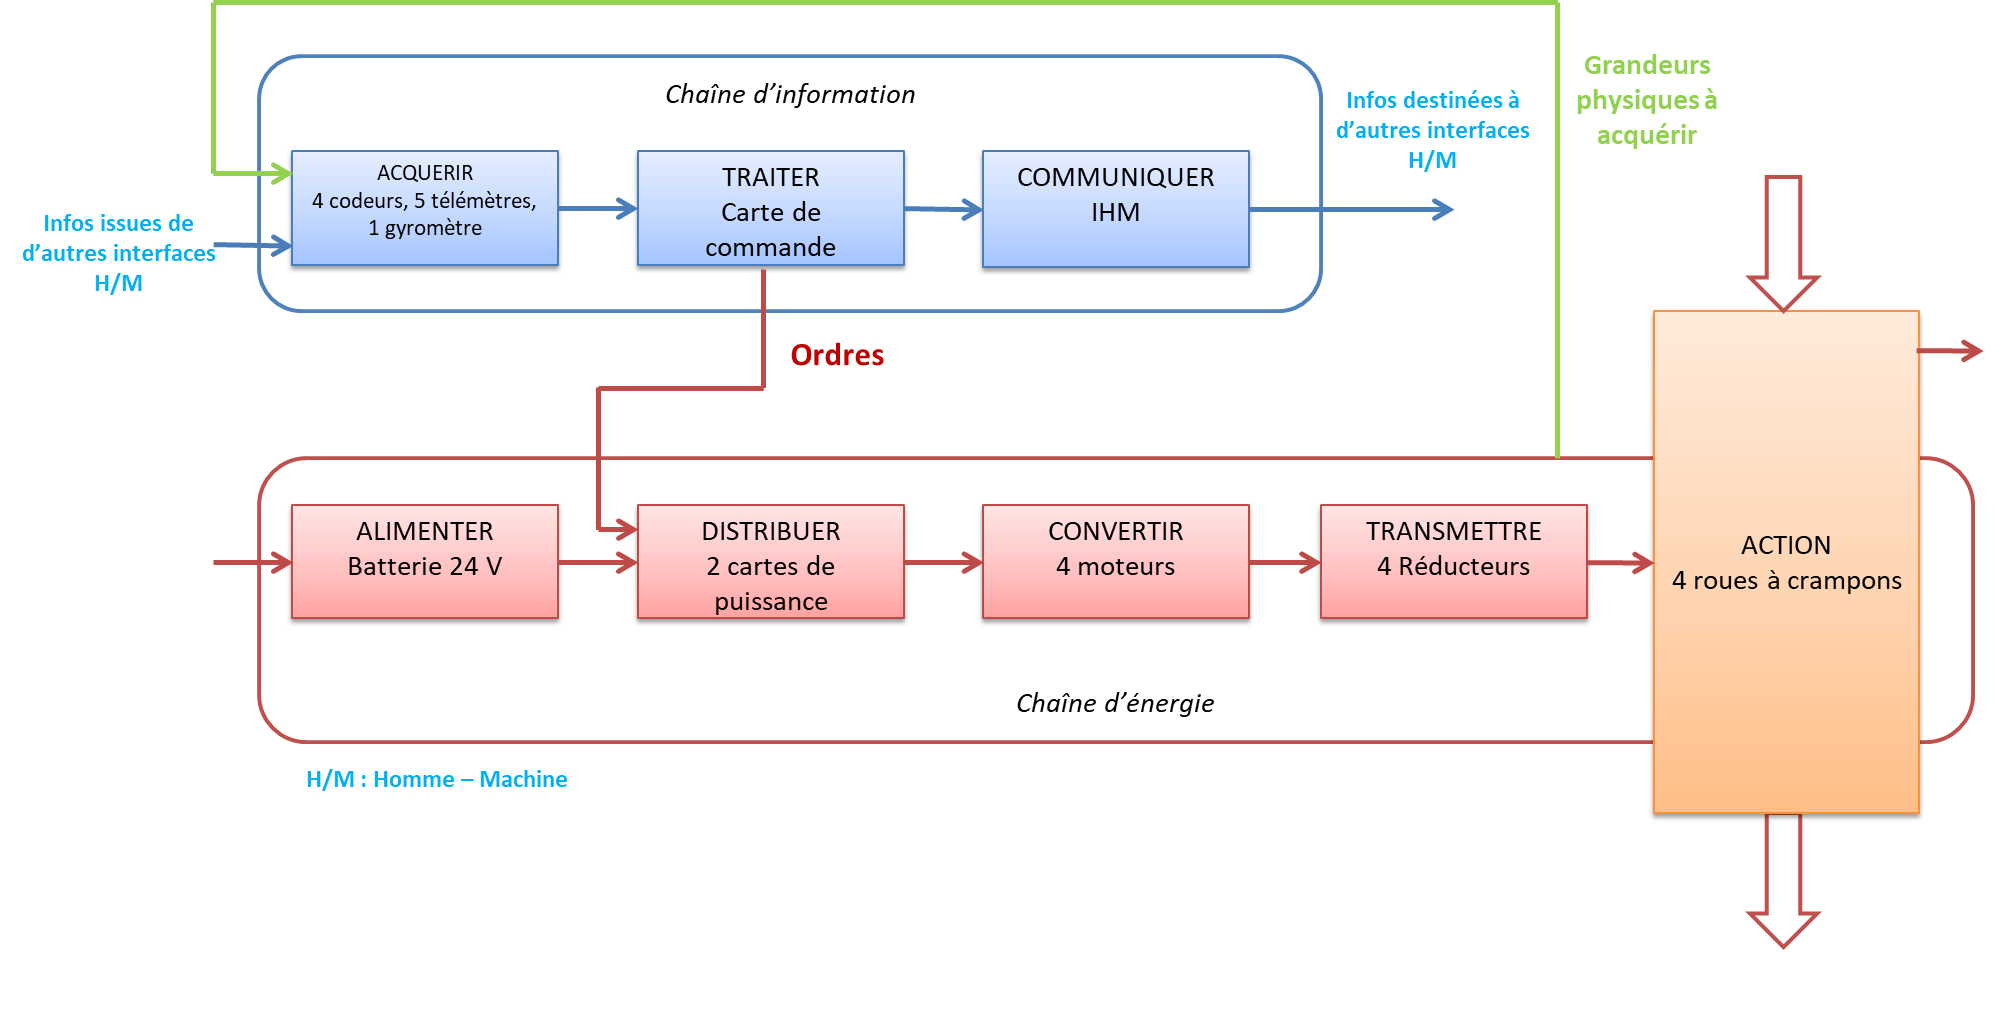
\includegraphics[width=\linewidth]{58_01_cor}
%\caption{Amplificateur de charge à plusieurs canaux KISTLER. \label{fig_50_01}}
\end{figure}

\else
\begin{flushright}
\footnotesize{Corrigé  voir \ref{SYS:01:58}.}
\end{flushright}%
\fi 
 
\graphicspath{{\repStyle/png/}{../SYS-01/SYS-01_ChaineFonctionnelle/59_Levage/images/}} 
\normaltrue \difficilefalse \tdifficilefalse
\correctionfalse

%\UPSTIidClasse{11} % 11 sup, 12 spé
%\newcommand{\UPSTIidClasse}{12}
% CCP MP 2011
\exer{Système de levage à multiples colonnes $\star$ \label{SYS:01:59}}
\setcounter{question}{0}\marginnote{\xpComp{SYS}{01}}
\index{Compétence SYS-01}
\index{Système de levage à multiples colonnes }
\index{Associer les fonctions aux constituants.}

\ifcorrection
\else
\marginnote{\textbf{Pas de corrigé pour cet exercice.}}
\fi

\ifprof
\else

Les sociétés de transports publics des grandes agglomérations gèrent des réseaux comportant des
bus et/ou des tramways. Ces sociétés possèdent des centres de maintenance ayant en charge
l’entretien et la réparation de leurs véhicules. %Parmi ces véhicules, on peut trouver des tramways de
%deux types : sur rails ou sur pneus. 
On s'intéresse ici à la maintenance de tramways sur rails de type
TFS (Tramway Français Standard).


Le système de levage est constitué d’une armoire de commande (nommée PC) munie d’un pupitre
de commande, d’un API (Automate Programmable Industriel), de relais et cartes de commande
pour moteurs. Cette PC peut gérer jusqu’à 10 colonnes de levage. Ces colonnes de levage sont des unités indépendantes mobiles que l’on peut déplacer manuellement
grâce à des roues escamotables. Elles sont constituées d’un chariot de levage guidé par 4 galets roulant à l’intérieur d’une colonne (rails
en tôle pliée). 


L’entraînement du chariot se fait par une vis à filet trapézoïdal, mise en rotation par un moto-réducteur-frein asynchrone. On met en place les colonnes au
niveau de la plate forme du tramway à soulever, aux endroits prévus à cet effet.


%\begin{multicols}{2}
\begin{figure}[H]
\centering
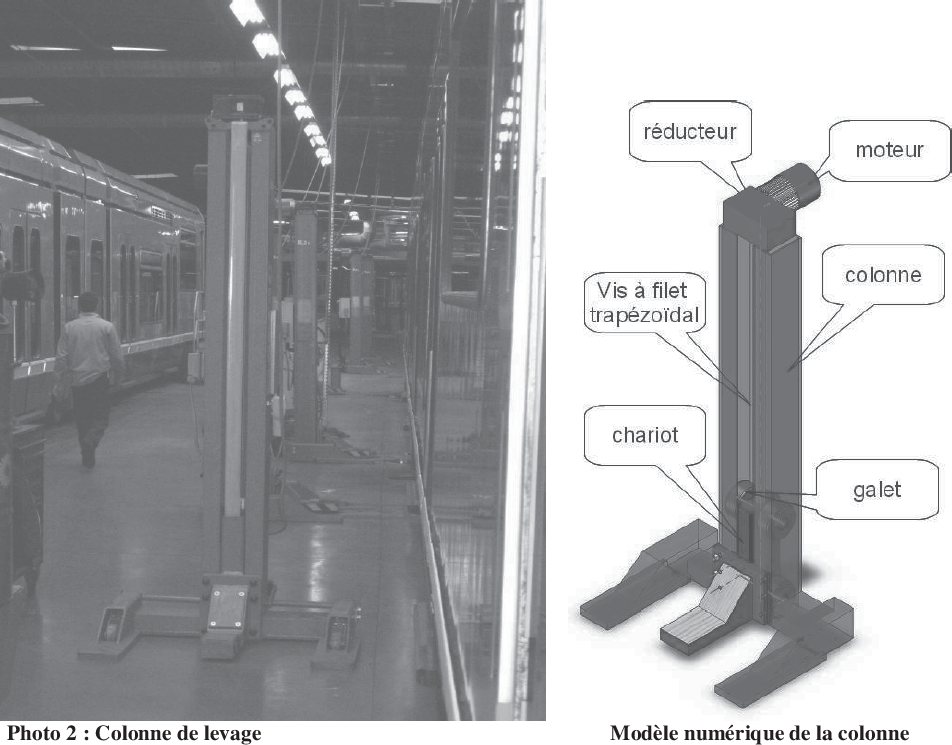
\includegraphics[height=4.5cm]{59_01}
%\caption{Amplificateur de charge à plusieurs canaux KISTLER. \label{fig_50_01}}
\end{figure}

\begin{figure}[H]
\centering
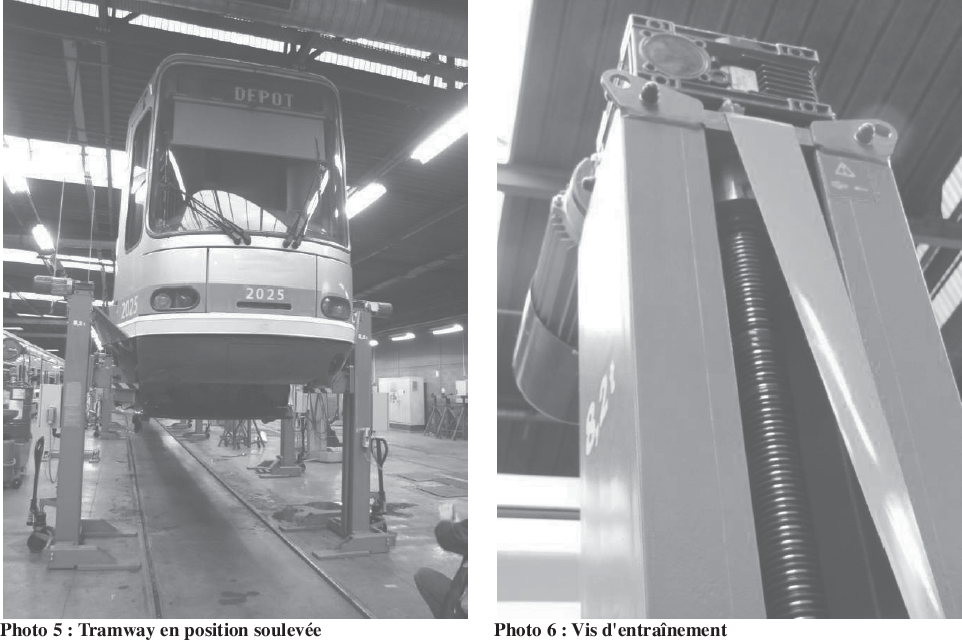
\includegraphics[height=4.5cm]{59_02}
\end{figure}

%\end{multicols}

Pour soulever un tramway de \SI{45}{tonnes} et de 30 mètres de long, le service de maintenance utilise 8
colonnes de levage d'une capacité unitaire maximale de 8,2 tonnes commandées simultanément. Lorsque les colonnes sont en place, on démarre le cycle de levage :
l’opérateur peut choisir un fonctionnement manuel ou automatique. En mode automatique, on
affiche sur le pupitre la consigne de hauteur à atteindre, la PC pilote alors chaque moteur des 8
colonnes jusqu’à ce que cette hauteur soit atteinte. Chaque colonne est équipée d’un codeur
incrémental informant la PC de la position du chariot de levage de la colonne. Pour un
fonctionnement en toute sécurité, il faut assurer une certaine horizontalité du tramway soulevé :
l'ensemble des points de levage doit être compris entre deux plans parallèles distants de \SI{20}{mm} au
maximum (coplanéité).



\begin{multicols}{2}

Le développement sous forme de FAST de la fonction principale F.P.1 (plus simplement écrite
« Soulever un tramway ») est donné ci-après.


\begin{figure}[H]
\centering
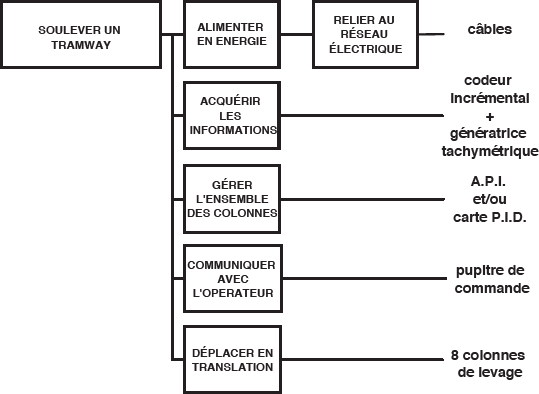
\includegraphics[height=4cm]{59_03}
\end{figure}

Le développement sous forme de FAST de la fonction technique « Déplacer en translation » pour
une colonne est donné ci-après.

\begin{figure}[H]
\centering
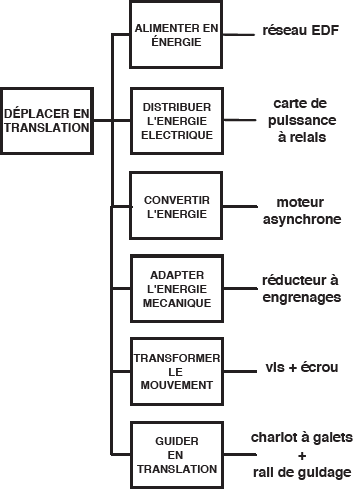
\includegraphics[height=4cm]{59_04}
\end{figure}
\end{multicols}

\fi

\question{Vous ne connaissez pas le diagramme FAST (je le sais). Quel(s) diagramme(s) SysML pourriez-vous utiliser pour remplacer les diagrammes << FAST >>.}

\question{Réaliser la chaîne fonctionnelle du système de levage étudié.}


\ifprof
\else
\begin{flushright}
\footnotesize{Corrigé  voir \ref{SYS:01:59}.}
\end{flushright}%
\fi 
 
\graphicspath{{\repStyle/png/}{../SYS-01/SYS-01_ChaineFonctionnelle/60_Escalier/images/}} 
\normaltrue \difficilefalse \tdifficilefalse
\correctionfalse

%\UPSTIidClasse{11} % 11 sup, 12 spé
%\newcommand{\UPSTIidClasse}{12}
% CCP MP 2014
\exer{Escalier mécanique$\star$ \label{SYS:01:60}}
\setcounter{question}{0}\xpComp{SYS}{01}
\index{Compétence SYS-01}
\index{Escalier mécanique}
\index{Associer les fonctions aux constituants.}

\ifcorrection
\else
\marginnote{\textbf{Pas de corrigé pour cet exercice.}}
\fi

\ifprof
\else


Un escalier mécanique (figure 1), appelé aussi escalier roulant ou Escalator (nom déposé par la société Otis), est un élévateur adapté au transport de personnes. Sa fonction principale est de faciliter le déplacement des piétons entre deux points de différentes hauteurs. 

%Depuis son invention en 1892 (à New York) par l’américain Jesse W. Reno, le système n’a pas cessé d’évoluer pour s’adapter aux nouvelles contraintes économiques, environnementales et sécuritaires.


\begin{figure}[H]
\centering
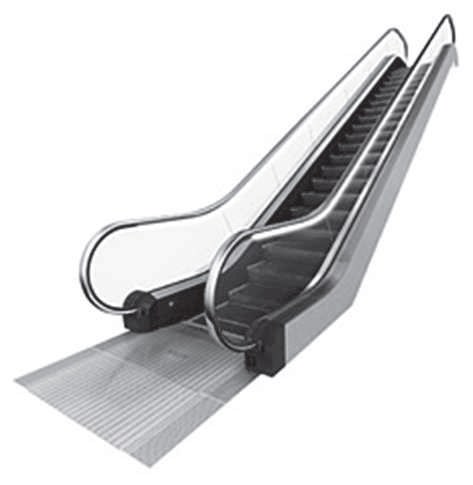
\includegraphics[width=4cm]{60_01}
%\caption{Amplificateur de charge à plusieurs canaux KISTLER. \label{fig_50_01}}
\end{figure}

%\ifprof
%\else
%\end{multicols}
\begin{figure}[H]
\centering
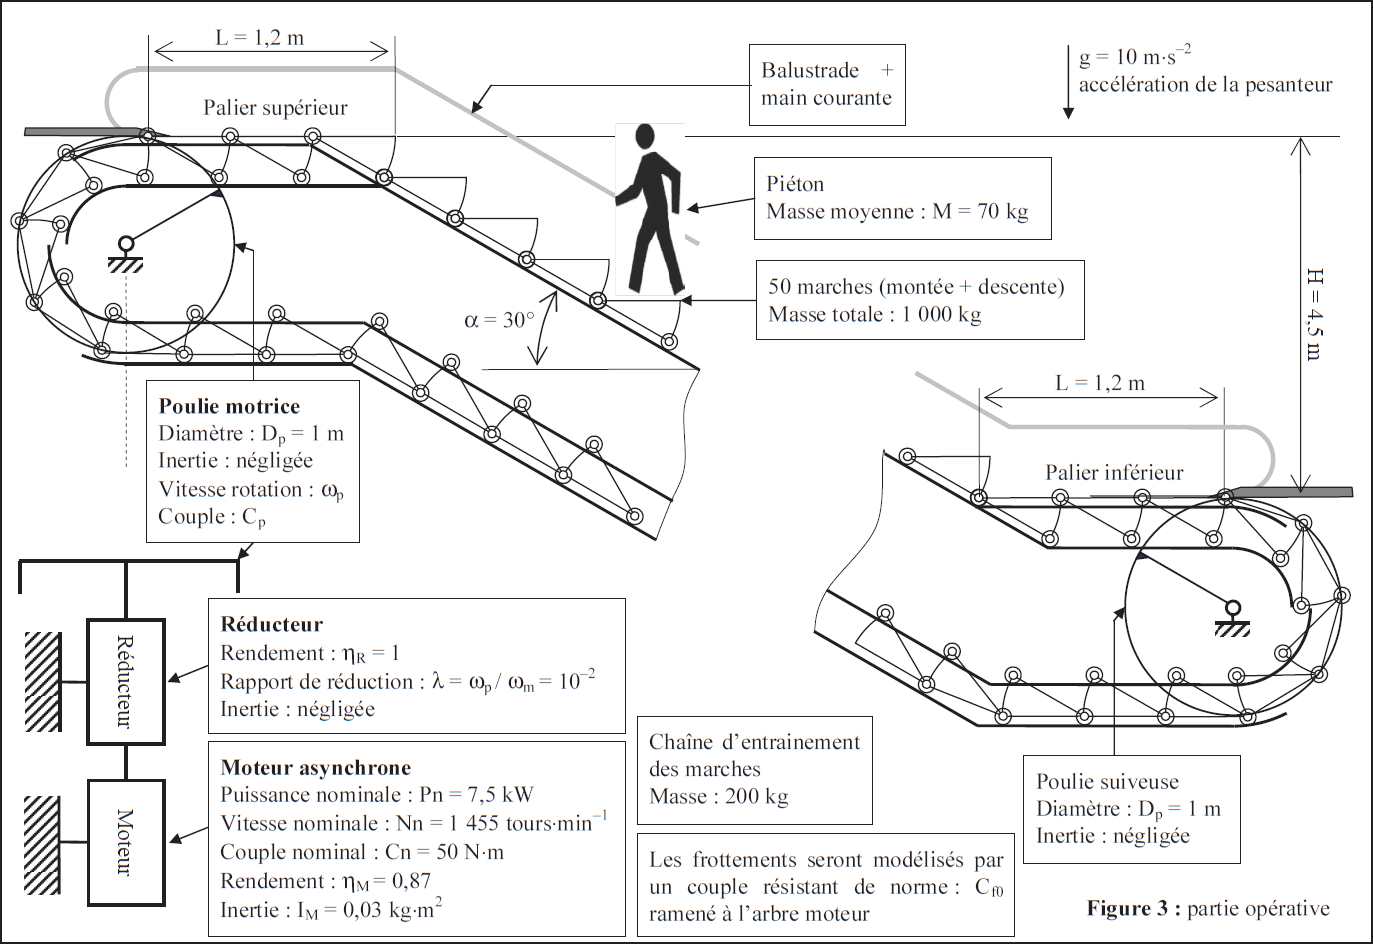
\includegraphics[width=\linewidth]{60_02}

\end{figure}
%\begin{multicols}{2}
\fi


\question{En analysant le schéma de principe de la figure précédente, proposer une chaîne fonctionnelle de l'escalier mécanique.}


\ifprof
\else
\begin{flushright}
\footnotesize{Corrigé  voir \ref{SYS:01:60}.}
\end{flushright}%
\fi 
 
\graphicspath{{\repStyle/png/}{../SYS-01/SYS-01_ChaineInfo/507_Divers/images/}} 
\normaltrue \difficilefalse \tdifficilefalse
\correctionfalse

%\UPSTIidClasse{11} % 11 sup, 12 spé
%\newcommand{\UPSTIidClasse}{12}
% ATS 2019
\exer{Capteurs $\star$ \label{SYS:01:507}}
\setcounter{question}{0}\xpComp{SYS}{01}
\index{Compétence SYS-01}
\index{Caractériser un constituant de la chaîne d’information.}
\index{Capteurs}
\ifcorrection
\else
\marginnote{\textbf{Pas de corrigé pour cet exercice.}}
\fi


\question{Donner le rôle et le principe de fonctionnement (schémas) des capteurs suivants : 
\begin{itemize}
\item génératrice tachymétrique;
\item potentiomètre rotatif;
\item codeur incrémental ;
\item codeur absolu. 
\end{itemize}.}
\ifprof
\else
\fi




\ifprof
\else
\begin{flushright}
\footnotesize{Corrigé  voir \ref{SYS:01:507}.}
\end{flushright}%
\fi 
 
\graphicspath{{\repStyle/png/}{../SYS-01/SYS-01_ChaineInfo/50_BancBalafre/images/}} 
\normaltrue \difficilefalse \tdifficilefalse
\correctionfalse

%\UPSTIidClasse{11} % 11 sup, 12 spé
%\newcommand{\UPSTIidClasse}{12}
% ATS 2019
\exer{Le banc balafre $\star$ \label{SYS:01:50}}
\setcounter{question}{0}\xpComp{SYS}{01}
\index{Compétence SYS-01}
\index{Le Banc Balafre}
\index{Caractériser un constituant de la chaîne d’information.}
\index{Capteurs}
\ifcorrection
\else
\marginnote{\textbf{Pas de corrigé pour cet exercice.}}
\fi

\ifprof
\else


Entre autres contrôles de la chaîne d’acquisition, le superviseur vérifie que la mesure des
efforts se fait correctement : au niveau des actionneurs piézoélectriques et au niveau du
joint testé. Les capteurs de force utilisés sur le système sont analogiques. Afin de simplifier
le traitement et l’interprétation de ces forces, on utilise un amplificateur de charges à
plusieurs canaux (voir figure \ref{fig_50_01}).





\begin{figure}[H]
\centering
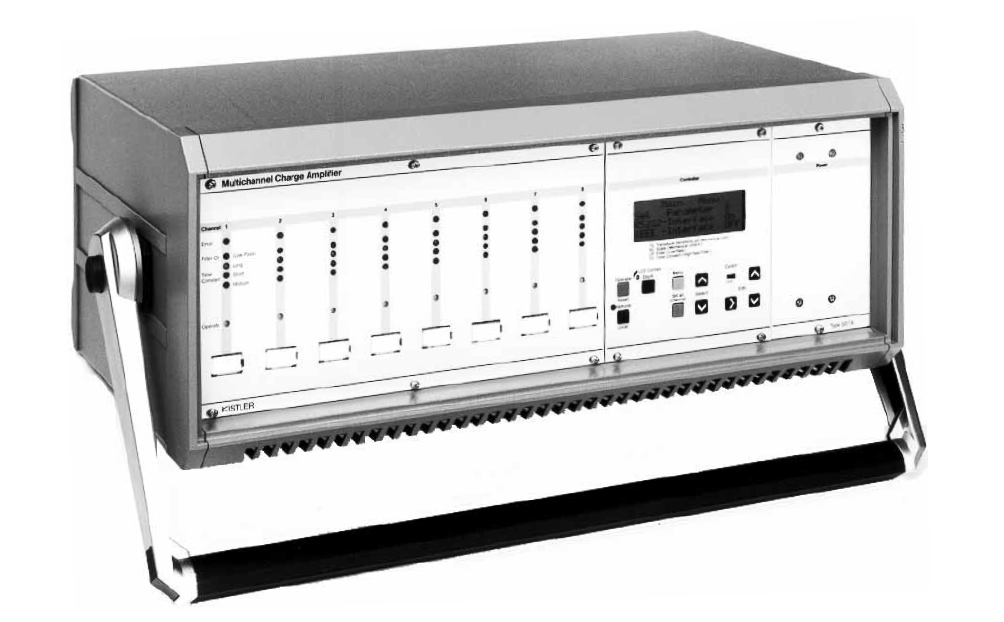
\includegraphics[width=\linewidth]{fig_50_01}
\caption{Amplificateur de charge à plusieurs canaux KISTLER. \label{fig_50_01}}
\end{figure}



Cet amplificateur possède deux options qui sont utilisées sur le banc Balafre :
\begin{itemize}
\item l’amplificateur de sommation pour le calcul analogique des forces et moments résultants
;
\item un convertisseur Analogique/Numérique pour faire le traitement des données (algorithme
de contrôle).
\end{itemize}
Dans l’algorithme de contrôle, la valeur d’effort de chaque actionneur est comparée à
la valeur théorique de la consigne effectuée pour le contrôle. Si un écart trop grand est
constaté, l’algorithme de contrôle émet un signal d’erreur (Controle=2). Pour cette mesure,
on considère qu’une résolution inférieure à  \SI{10}{N} est nécessaire.
La conversion analogique/numérique se fait ici sur 12 bits. La mesure de l’effort se fait
sur la plage de $-20$ à \SI{20}{kN}. Les données techniques utiles sont rassemblées sur la figure
\ref{fig_50_02}.

Le capteur de force (voir figure \ref{fig_50_03}) utilisé est un capteur KISTLER 9167A, permettant
de mesurer des efforts dans trois directions. Pour la mesure de l’effort développé par
les actionneurs, seule la direction Z est utilisée, et la sensibilité du capteur dans cette
direction est \SI{4,2}{pC.N^{-1}}.
Le synoptique de la figure \ref{fig_50_04} présente la structure interne de l’amplificateur de charge.

\begin{figure}[H]
\centering
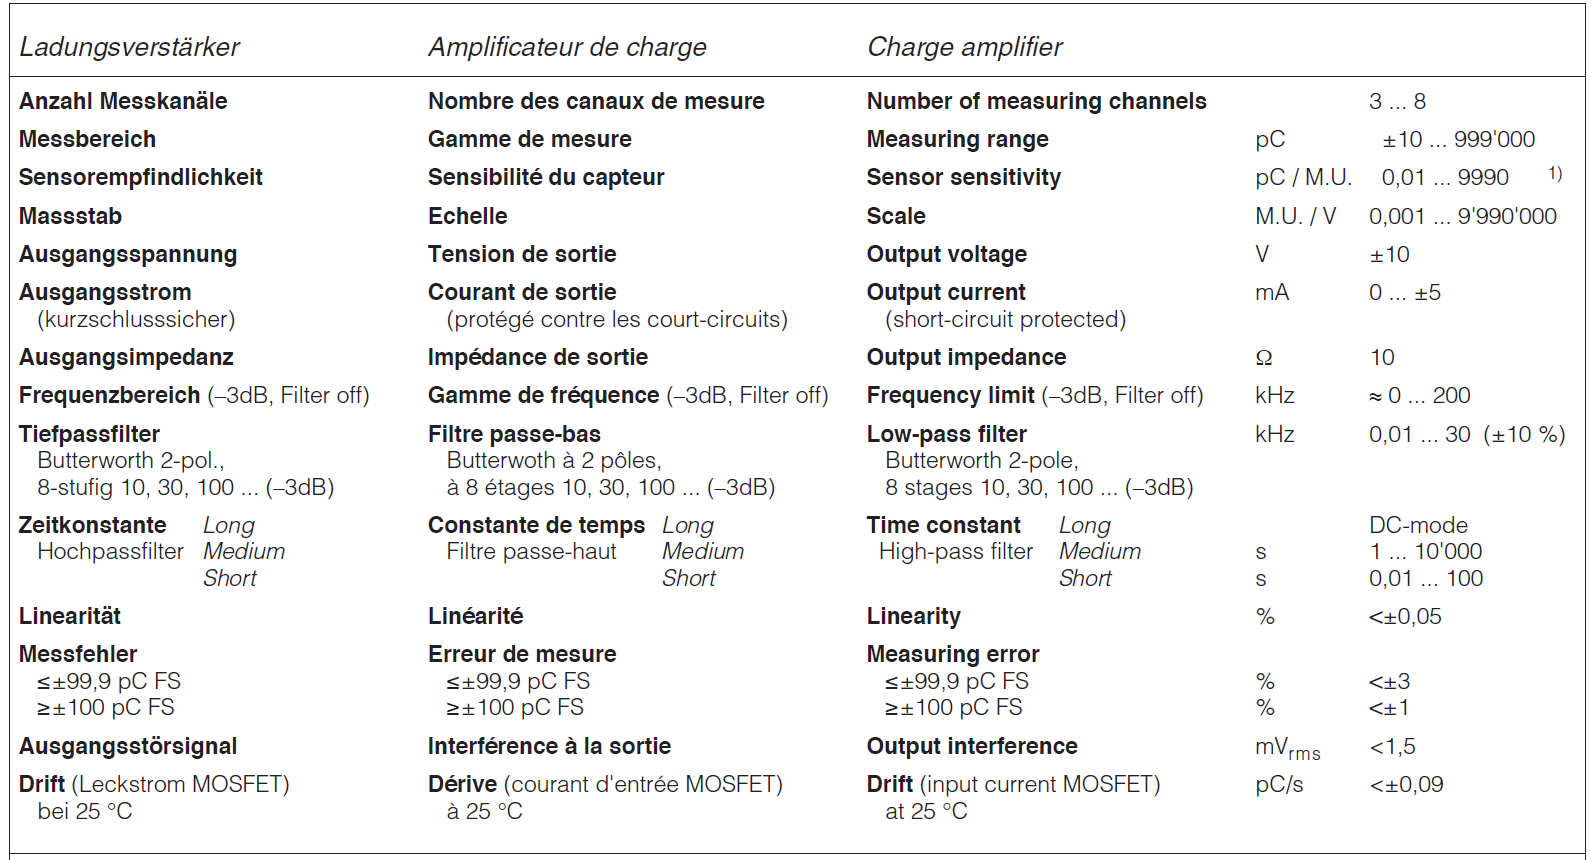
\includegraphics[width=\linewidth]{fig_50_02}
\caption{Amplificateur de charge à plusieurs canaux KISTLER. \label{fig_50_02}}
\end{figure}


\begin{figure}[H]
\centering
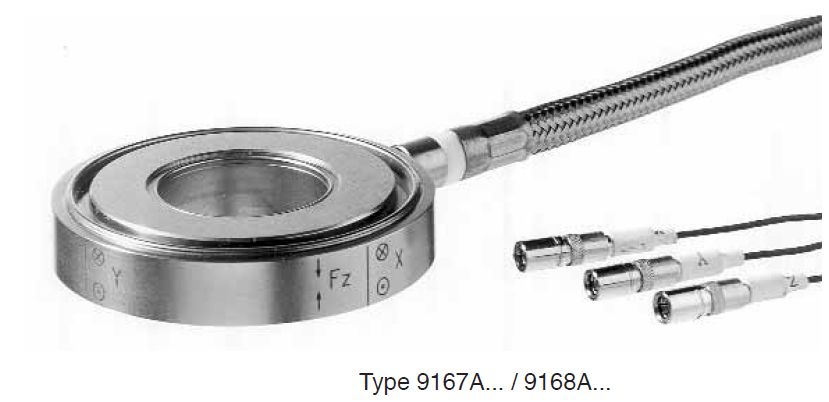
\includegraphics[width=.7\linewidth]{fig_50_03}
\caption{Capteur de force KISTLER 9167A. \label{fig_50_03}}
\end{figure}

\begin{figure}[H]
\centering
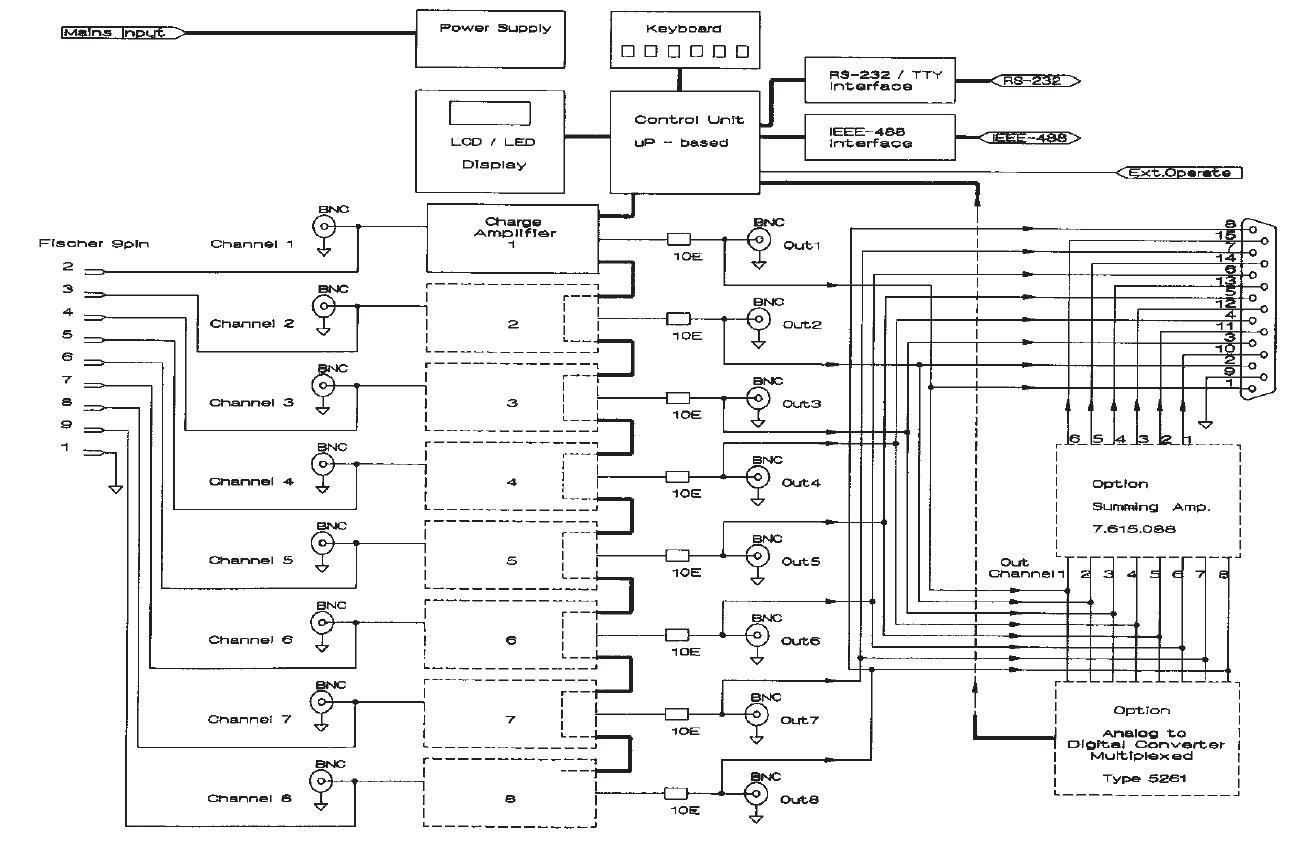
\includegraphics[width=\linewidth]{fig_50_04}
\caption{Synoptique de la structure interne de l’amplificateur de charge. \label{fig_50_04}}
\end{figure}
\fi

\question{Sur le synoptique de la figure \ref{fig_50_04}, on peut lire « Analog to Digital
Converter Multiplexed ». Que signifie le terme multiplexé utilisé ici ?}
\ifprof
\else
\fi

\question{Compte tenu de la sensibilité du capteur et de l’étendue des valeurs à
mesurer, déterminer la gamme de mesure à régler sur l’amplificateur de charge.}
\ifprof
\else
\fi

\question{En utilisant la documentation technique de l’amplificateur de charge,
déterminer la plage de variation de la tension de sortie de l’amplificateur. En déduire le
quantum de la conversion analogique numérique, puis la résolution de la mesure. Conclure
vis-à-vis de la résolution demandée.}
\ifprof
\else
\fi




\ifprof
\else
\begin{flushright}
\footnotesize{Corrigé  voir \ref{SYS:01:50}.}
\end{flushright}%
\fi 
 
\graphicspath{{\repStyle/png/}{../SYS-01/SYS-01_ChaineInfo/538_Codeur/images/}} 
\normaltrue \difficilefalse \tdifficilefalse
\correctionfalse

%\UPSTIidClasse{11} % 11 sup, 12 spé
%\newcommand{\UPSTIidClasse}{12}
% ATS 2019
\exer{Codeur incrémental $\star$ \label{SYS:01:538}}
\setcounter{question}{0}\marginnote{\xpComp{SYS}{01}}
\index{Compétence SYS-01}
\index{Caractériser un constituant de la chaîne d’information.}
\index{Capteurs}
\ifcorrection
\else
\marginnote{\textbf{Pas de corrigé pour cet exercice.}}
\fi

\begin{marginfigure}
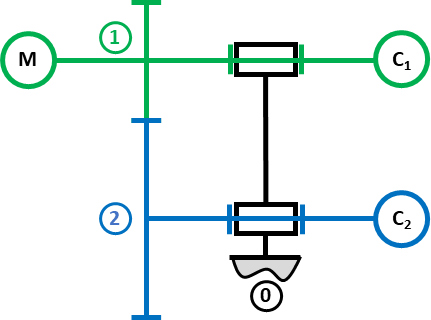
\includegraphics[width=5cm]{538_01}
\end{marginfigure}

\question{Donner le rôle et le principe de fonctionnement (schémas) d'un codeur incrémental optique.}
\ifprof
\else
\fi

\question{Le codeur est équipé d'une voie de mesure et d'un disque à 25 fentes. Donner la résolution du capteur en degtés.}
\ifprof
\else
\fi

\question{Quelle sera la résolution du capteur s'il est équipé de deux voies de mesure ?}
\ifprof
\else
\fi

\ifprof
\else
Un codeur est monté en sortie d'un moteur. Le moteur est suivi d'un réducteur de rapport 100.

\fi

\question{Quelle est la résolution du capteur vis-à-vis de l'arbre de sortie du réducteur ?}
\ifprof
\else
\fi

\ifprof
\else
La position du codeur est transformée par un convertisseur numérique analogique en V. Ce convertisseur permet de convertir des angles variants de $-$10 tours à +10 tours sur une échelle de $-5$ à +\SI{5}{V}.   
\fi

\question{Donner le gain du convertisseur numérique analogique.}
\ifprof
\else
\fi


\ifprof
\else
\begin{flushright}
\footnotesize{Corrigé  voir \ref{SYS:01:538}.}
\end{flushright}%
\fi 
 
\graphicspath{{\repStyle/png/}{../SYS-01/SYS-01_ChainePuissance/1100_Pneumatique/images/}} 
\normaltrue \difficilefalse \tdifficilefalse
\correctionfalse

%\UPSTIidClasse{11} % 11 sup, 12 spé
%\newcommand{\UPSTIidClasse}{12}
% ATS 2019
\exer{Vérin double effets $\star$ \label{A3:05:1100}}
\setcounter{question}{0}\marginnote{\xpComp{SYS}{01}}
\index{Compétence A3-05}
\index{Distributeur}
\index{Vérin}
\ifcorrection
\else
\marginnote{\textbf{Pas de corrigé pour cet exercice.}}
\fi


Un vérin double effet est commandé par un distributeur 4/2 (4 orifices, 2 positions) bi-stable.



\ifprof
\else
%\begin{marginfigure}
%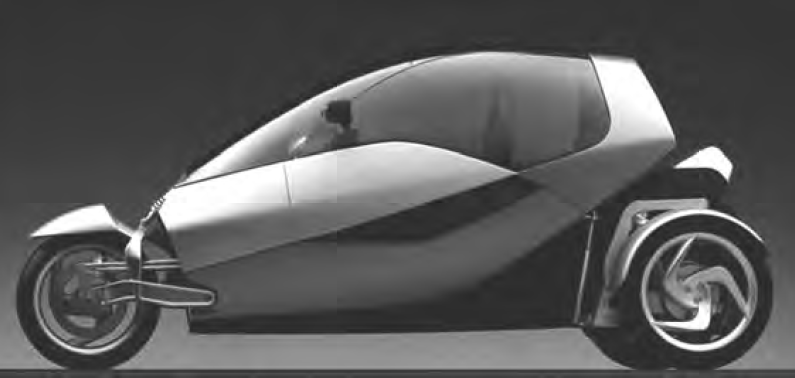
\includegraphics[width=.8\linewidth]{fig_80_01}
%%\textit{}
%\end{marginfigure}




\begin{marginfigure}
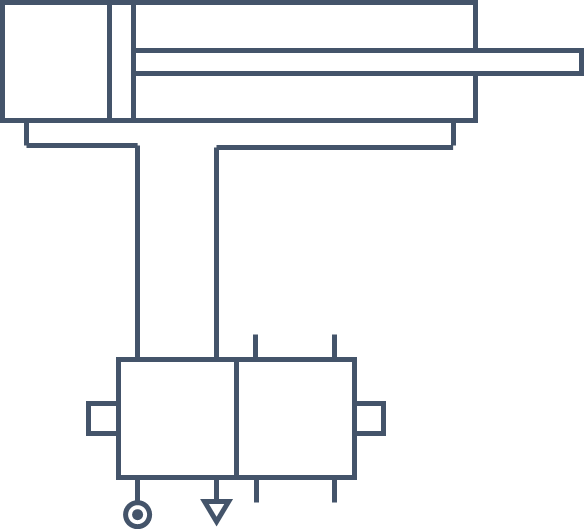
\includegraphics[width=\linewidth]{1100_fig_01}
%\textit{}
\end{marginfigure}

\question{Compléter le câblage du distributeur.}

\question{Dans la position actuelle, indiquer par des flèches le sens de déplacement du vérin. Indiquer en rouge les tuyaux et chambre hautes pressions. Indiquer en bleu les tuyaux et chambre basses pressions.}

\question{On souhaite ralentir le déplacement du vérin lorsqu'il sort de la chambre. Positionner le limiteur de débit en conséquence.}

\begin{marginfigure}
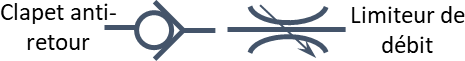
\includegraphics[width=\linewidth]{1100_fig_02}
%\textit{}
\end{marginfigure}


\question{Ajouter un clapet anti-retour pour éviter la limitation du débit lorsque le vérin se rétracte.}



\ifprof
\begin{corrige}
\begin{center}
%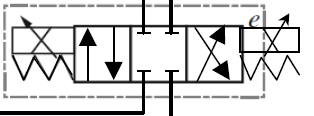
\includegraphics[width=.5\linewidth]{fig_80_cor_01}
%\textit{}
\end{center}
\end{corrige}
\else\begin{center}
%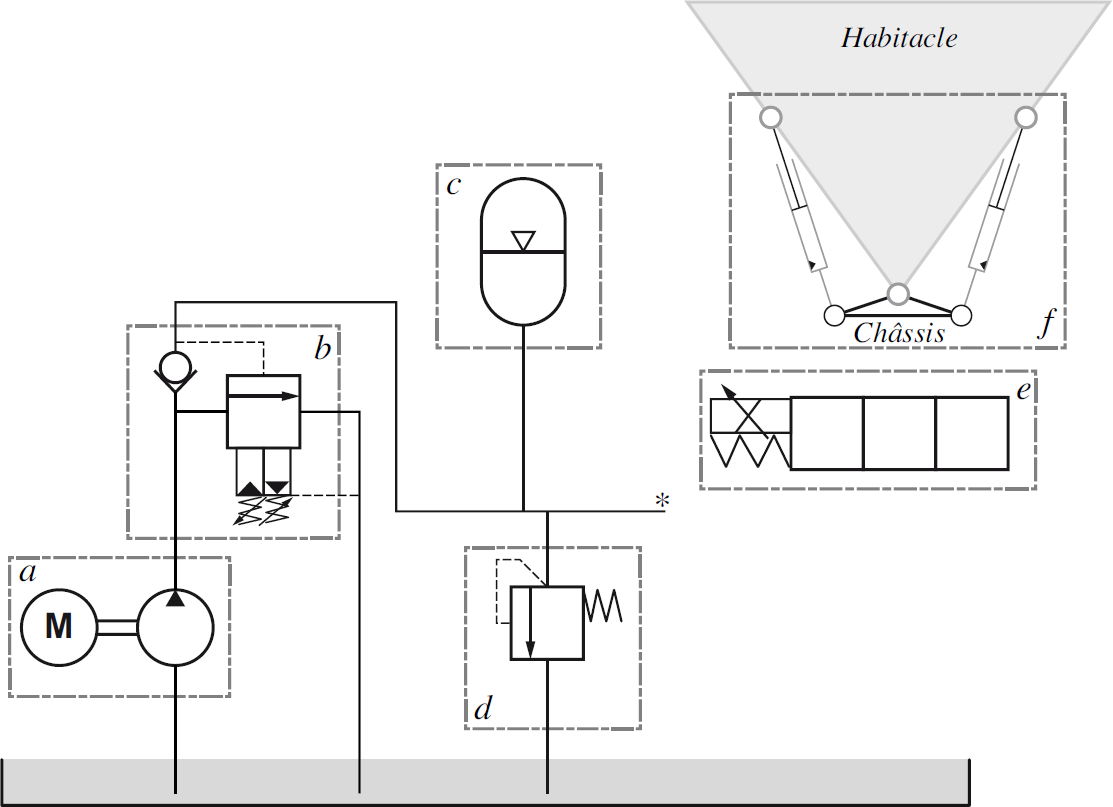
\includegraphics[width=\linewidth]{fig_80_05}
%\textit{}
\end{center}

\fi

Au démarrage du véhicule, la valve de décharge du module (b) est fermée. Le distributeur à effet proportionnel(e) est en position médiane, les vérins sont donc immobiles. La commande des vérins est initialement bloquée par une temporisation.

\question{En considérant les conditions initiales évoquées, expliquer, en commençant à l’instant de démarrage de la pompe, le comportement du circuit hydraulique en précisant clairement les différentes phases de fonctionnement. Quel est l’utilité de la temporisation ? On souhaite remplacer cette temporisation par un capteur. Préciser la grandeur qu’il devra mesurer. Donner un avantage et un inconvénient du remplacement de la temporisation par ce capteur.}
\ifprof
\begin{corrige}
Démarrage de la pompe et montée en pression du circuit avec remplissage de l’accumulateur (c).

À la fin de la temporisation le distributeur peut être commandé et ainsi alimenter les vérins.

Si la pression augmente trop, alors le limiteur de pression (d) renvoie une partie du fluide vers le
réservoir et si c’est insuffisant alors (b) permet une décharge du circuit (ouverture vers le réservoir
jusqu’à atteindre ne niveau bas réglé).

La temporisation permet d’attendre qu’un niveau de pression suffisant dans le circuit soit atteint.

Pour remplacer la temporisation on peut mesurer la pression dans le circuit ou plus simplement détecter
le niveau de pression satisfaisant pour le fonctionnement à l’aide d’un pressostat.

La solution utilisant un capteur de pression est plus sûre que la temporisation qui pourrait autoriser la
commande du distributeur alors que la pression dans le circuit est encore insuffisante.

(UPSTI). 
\end{corrige}
\else
\fi






\ifprof
\else
\begin{flushright}
\footnotesize{Corrigé  voir \ref{A3:05:80}.}
\end{flushright}%
\fi 
 
\graphicspath{{\repStyle/png/}{../SYS-01/SYS-01_ChainePuissance/80_Clever/images/}} 
\normaltrue \difficilefalse \tdifficilefalse
\correctionfalse

%\UPSTIidClasse{11} % 11 sup, 12 spé
%\newcommand{\UPSTIidClasse}{12}
% ATS 2019
\exer{Véhicule à trois roues Clever $\star$ \label{A3:05:80}}
\setcounter{question}{0}%\marginnote{\xpComp{SYS}{01}}
\marginnote{\index{Compétence A3-05}}
\index{Véhicule à trois roues Clever}
\index{Caractériser un constituant de la chaîne de puissance.}
\index{Distributeur}
\index{Vérin}
\ifcorrection
\else
\marginnote{\textbf{Pas de corrigé pour cet exercice.}}
\fi




On s'intéresse au véhicule à 3 roues Clever.

\ifprof
\else
%\begin{marginfigure}
%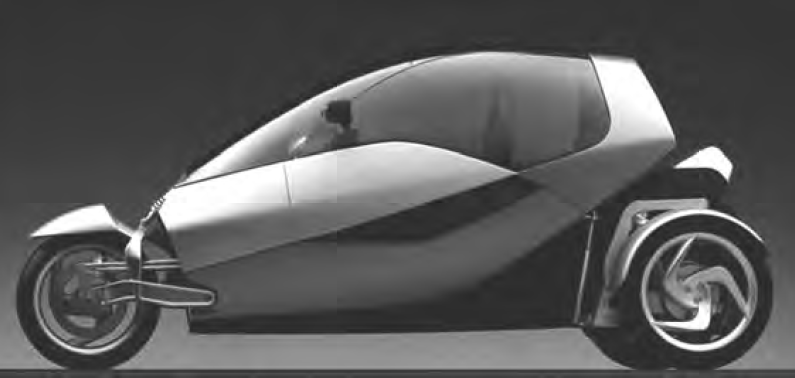
\includegraphics[width=.8\linewidth]{fig_80_01}
%%\textit{}
%\end{marginfigure}


 Le groupe motopropulseur est placé à l'arrière du véhicule. À l’avant, l’habitacle repose sur une roue de moto et pivote par rapport au bloc arrière autour d’une liaison pilotée angulairement par le biais de deux vérins hydrauliques. L'inclinaison est contrôlée par un ordinateur de bord en fonction de l'angle au volant et de la vitesse. 

\begin{marginfigure}
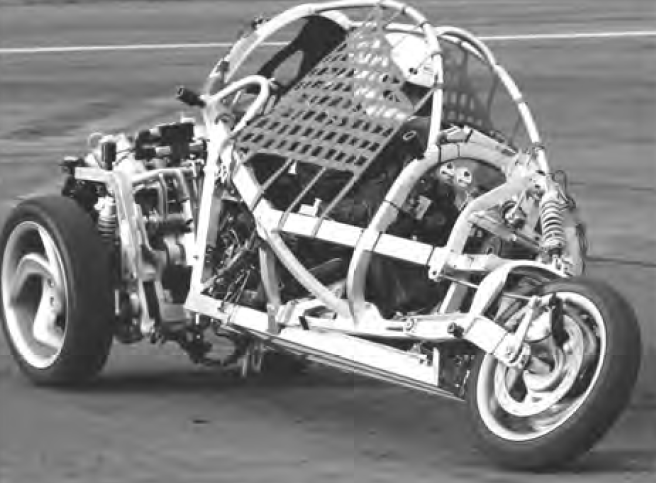
\includegraphics[width=\linewidth]{fig_80_02}
%\textit{}
\end{marginfigure}

%Le système d’inclinaison de l’habitacle est assuré par un système constitué :
%\begin{itemize}
%\item d’un calculateur qui détermine le mouvement et la position à donner à l’habitacle en fonction des conditions
%d’utilisation;
%\item d’un système hydro-mécanique de transmission de puissance et d’adaptation de mouvement;
%\item d’un système de contrôle de l’inclinaison de l’habitacle.
%\end{itemize}

La chaîne de transmission de puissance et d’adaptation de mouvement est composée :
\begin{itemize}
\item d’une pompe à engrenages actionnée par le moteur à gaz via un système de poulies/courroie;
\item d’un circuit hydraulique;
\item de 2 vérins hydrauliques simple effet;
\item d’un système mécanique d’adaptation de mouvement afin de transformer le mouvement de translation des tiges des vérins en rotation de l’habitacle.
\end{itemize}


\begin{center}
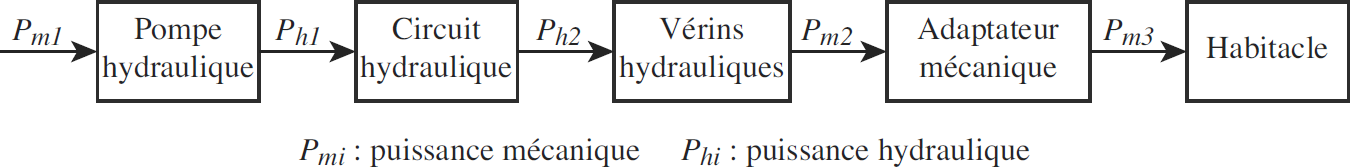
\includegraphics[width=\linewidth]{fig_80_03}
%\textit{}
\end{center}

\begin{center}
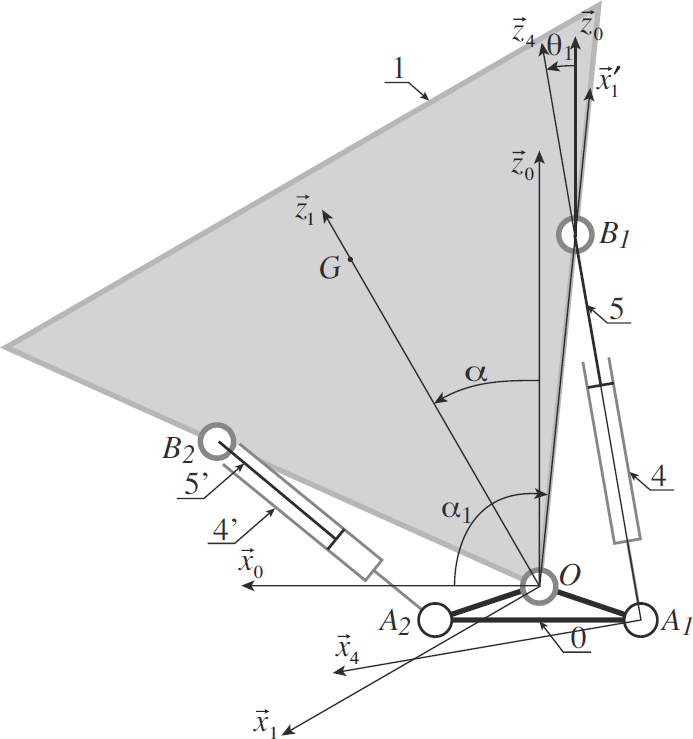
\includegraphics[width=.7\linewidth]{fig_80_04}
%\textit{}
\end{center}


Les deux vérins hydrauliques transforment la puissance hydraulique venant du servo-distributeur afin d’incliner l’habitacle. Ceux-ci sont disposées entre l’habitacle et le châssis du module arrière de propulsion. Le calculateur autorise ou non, l’alimentation en huile de l’un des vérins provoquant la sortie de tige, pendant que l’huile s'évacue de l’autre vérin. Ainsi l’habitacle s'incline du coté opposée au vérin alimenté. Lorsque l’habitacle est en position centrale, les tiges de vérins ont en position médiane.


Le circuit hydraulique est composé de 6 modules:
\begin{itemize}
\item une pompe à engrenages entraînée par le moteur à gaz;
\item un clapet anti-retour et une valve de décharge tarée pour s’enclencher à \SI{160}{bar} et se remettre en position fermée à \SI{100}{bar};
\item un accumulateur oléopneumatique de volume nominal \SI{1,4}{L};
\item un limiteur de pression;
\item un servo-distributeur à effet proportionnel 4/3 à centre fermé;
\item deux vérins simple effet, de diamètre \SI{32}{mm} pour chaque piston et de \SI{200}{mm} de course.
\end{itemize}

\fi

\question{Compléter le câblage du circuit hydraulique à partir du signe << * >>, ainsi que le schéma  du servo-distributeur.}

\ifprof
\begin{corrige}
\begin{center}
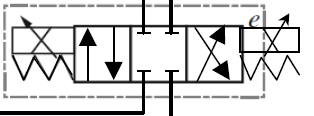
\includegraphics[width=.5\linewidth]{fig_80_cor_01}
%\textit{}
\end{center}
\end{corrige}
\else\begin{marginfigure}
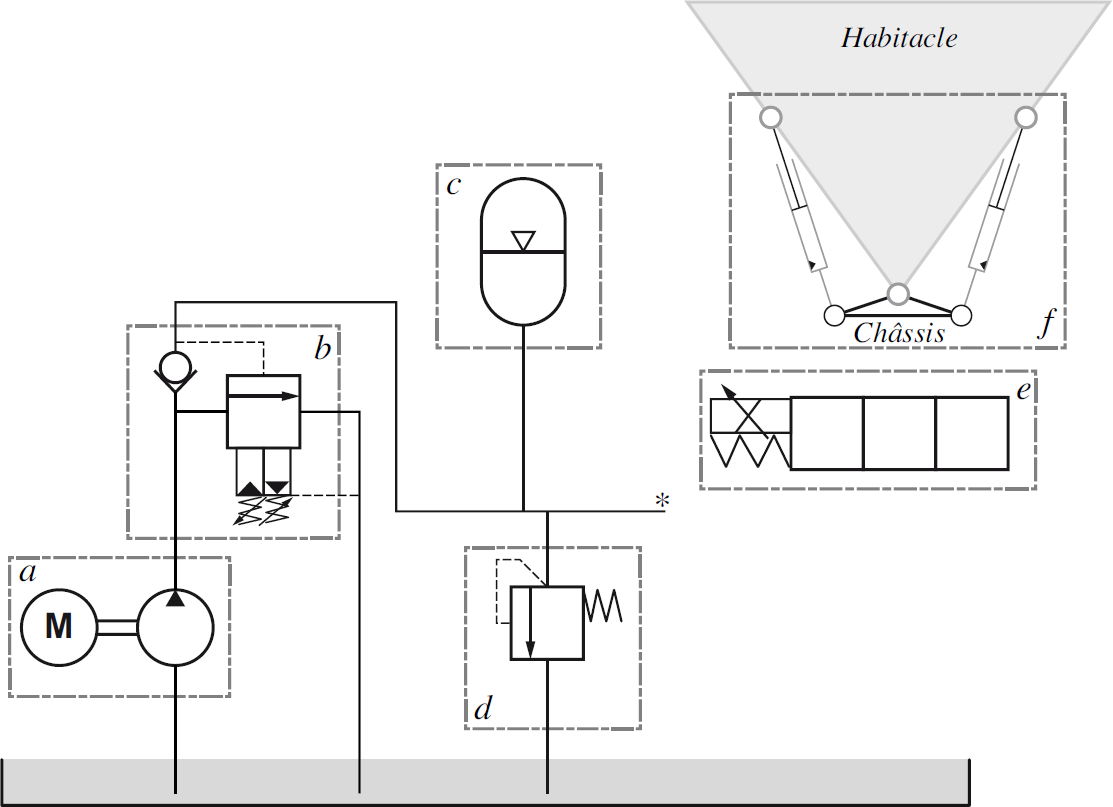
\includegraphics[width=\linewidth]{fig_80_05}
%\textit{}
\end{marginfigure}

\fi

Au démarrage du véhicule, la valve de décharge du module (b) est fermée. Le distributeur à effet proportionnel(e) est en position médiane, les vérins sont donc immobiles. La commande des vérins est initialement bloquée par une temporisation.

\question{En considérant les conditions initiales évoquées, expliquer, en commençant à l’instant de démarrage de la pompe, le comportement du circuit hydraulique en précisant clairement les différentes phases de fonctionnement. Quel est l’utilité de la temporisation ? On souhaite remplacer cette temporisation par un capteur. Préciser la grandeur qu’il devra mesurer. Donner un avantage et un inconvénient du remplacement de la temporisation par ce capteur.}
\ifprof
\begin{corrige}
Démarrage de la pompe et montée en pression du circuit avec remplissage de l’accumulateur (c).

À la fin de la temporisation le distributeur peut être commandé et ainsi alimenter les vérins.

Si la pression augmente trop, alors le limiteur de pression (d) renvoie une partie du fluide vers le
réservoir et si c’est insuffisant alors (b) permet une décharge du circuit (ouverture vers le réservoir
jusqu’à atteindre ne niveau bas réglé).

La temporisation permet d’attendre qu’un niveau de pression suffisant dans le circuit soit atteint.

Pour remplacer la temporisation on peut mesurer la pression dans le circuit ou plus simplement détecter
le niveau de pression satisfaisant pour le fonctionnement à l’aide d’un pressostat.

La solution utilisant un capteur de pression est plus sûre que la temporisation qui pourrait autoriser la
commande du distributeur alors que la pression dans le circuit est encore insuffisante.

(UPSTI). 
\end{corrige}
\else
\fi






\ifprof
\else
\begin{flushright}
\footnotesize{Corrigé  voir \ref{A3:05:80}.}
\end{flushright}%
\fi 
 
\graphicspath{{\repStyle/png/}{../SYS-01/SYS-01_ChainePuissance/88_Suspension/images/}} 
\normaltrue \difficilefalse \tdifficilefalse
\correctionfalse

%\UPSTIidClasse{11} % 11 sup, 12 spé
%\newcommand{\UPSTIidClasse}{12}
% ATS 2019
\exer{Suspension pneumatique de véhicule de transport routier$\star$ \label{A3:05:88}}
\setcounter{question}{0}\UPSTIcompetence[2]{A3-05}
\index{Compétence A3-05}
\index{Suspension pneumatique}
\index{Caractériser un constituant de la chaîne de puissance.}
\index{Distributeur}
\index{Vérin}
\ifcorrection
\else
\marginnote{\textbf{Pas de corrigé pour cet exercice.}}
\fi



\ifprof
\else
La suspension assure la liaison élastique entre le châssis et les essieux. Elle permet principalement d’atténuer les accélérations verticales dues aux variations de profil de la chaussée, contribuant ainsi à l’amélioration du confort et à une meilleure tenue de route.

\begin{center}
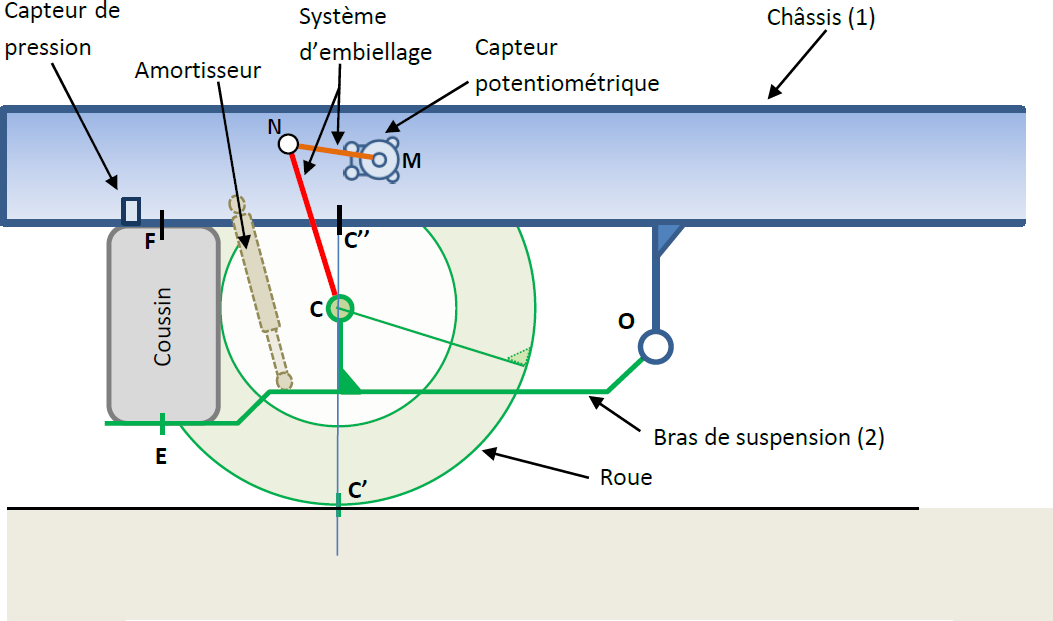
\includegraphics[width=\linewidth]{88_fig_01}
%\textit{}
\end{center}

Chaque roue possède une suspension pneumatique sur coussin pilotée par des électrovannes, en fonction de données mesurées par des capteurs de pression et des capteurs de position. Un calculateur envoie des commandes électriques aux électrovannes en fonction des besoins.

\begin{center}
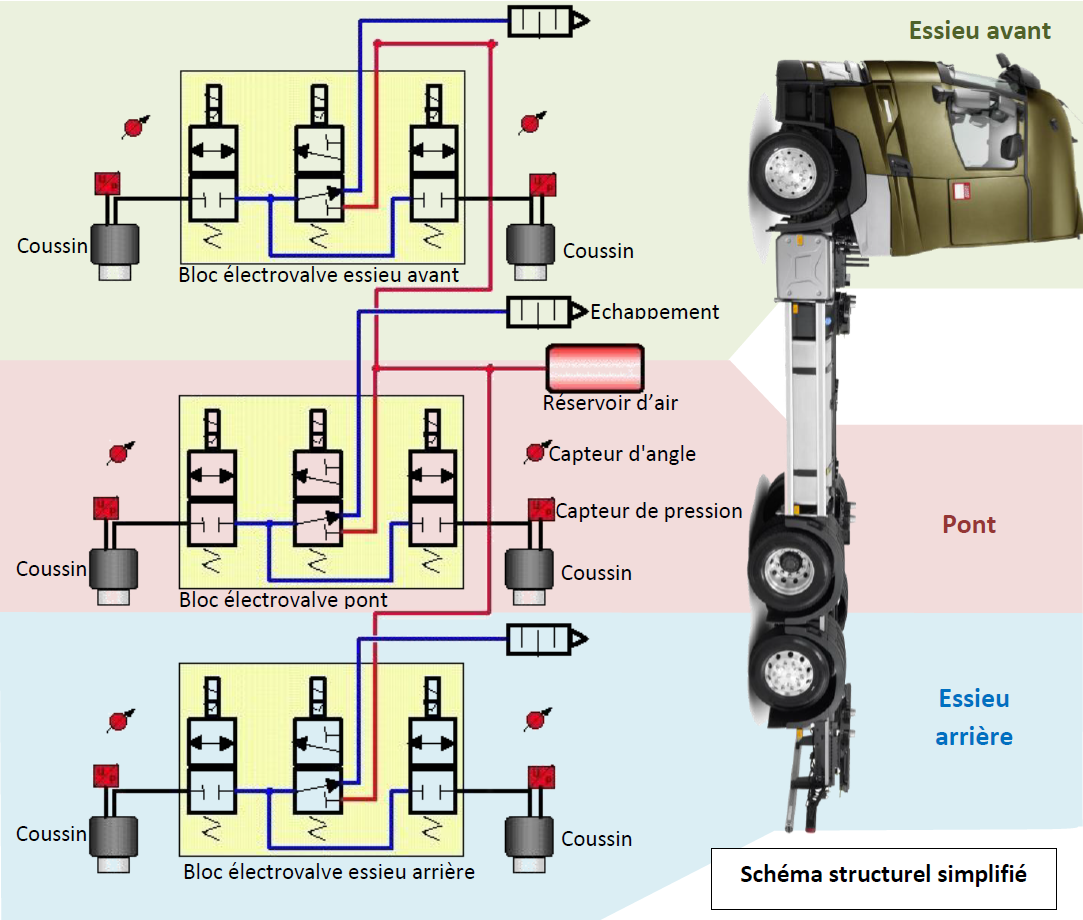
\includegraphics[width=\linewidth]{88_fig_02}
%\textit{}
\end{center}


\begin{center}
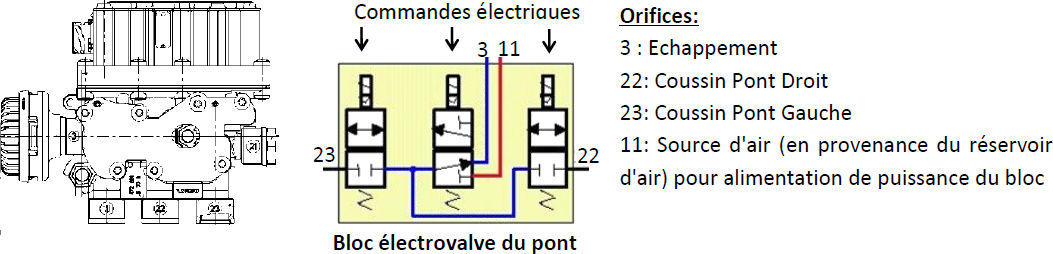
\includegraphics[width=\linewidth]{88_fig_03}
%\textit{}
\end{center}

Lorsque le niveau mesuré est inférieur à la valeur de consigne (niveau du châssis par rapport au sol), l’électrovalve est commandée de manière à provoquer le gonflage des coussins.
Lorsque le niveau a dépassé la consigne, on commande la vidange des coussins.

\fi
\question{Représenter les trois distributeurs dans la situation de gonflage, puis dans la situation de vidange des coussins.
}
\ifprof
\begin{corrige}
\begin{center}
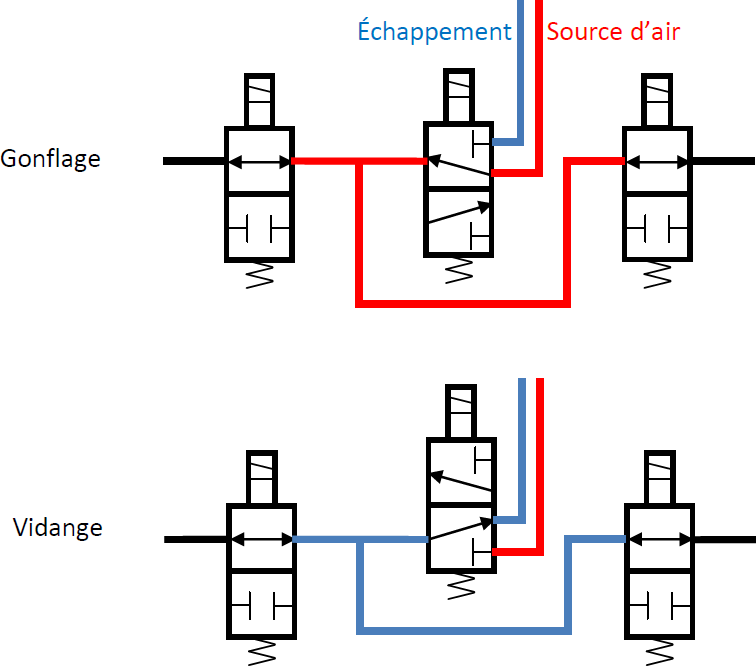
\includegraphics[width=.5\linewidth]{88_cor_01}
%\textit{}
\end{center}
\end{corrige}
\else
\fi







\ifprof
\else
\begin{flushright}
\footnotesize{Corrigé  voir \ref{A3:05:88}.}
\end{flushright}%
\fi 
 
\graphicspath{{\repStyle/png/}{../SYS-01/SYS-01_ChainePuissance/89_Bouee/images/}} 
\normaltrue \difficilefalse \tdifficilefalse
\correctionfalse

%\UPSTIidClasse{11} % 11 sup, 12 spé
%\newcommand{\UPSTIidClasse}{12}
% ATS 2019
\exer{Suspension pneumatique de véhicule de transport routier$\star$ \label{A3:05:89}}
\setcounter{question}{0}
\marginnote{\xpComp{SYS}{01}}%\UPSTIcompetence[2]{A3-05}

\index{Compétence A3-05}
\index{Compétence SYS-01}
\index{Bouée}
\index{Caractériser un constituant de la chaîne de puissance}
\index{Distributeur}
\index{Vérin}
\ifcorrection
\else
\marginnote{\textbf{Pas de corrigé pour cet exercice.}}
\fi



\ifprof
\else
L’énergie produite à partir de la houle est appelée houlomotrice (ou énergie des vagues). Cette énergie est le plus souvent
transformée en énergie électrique.

\begin{marginfigure}
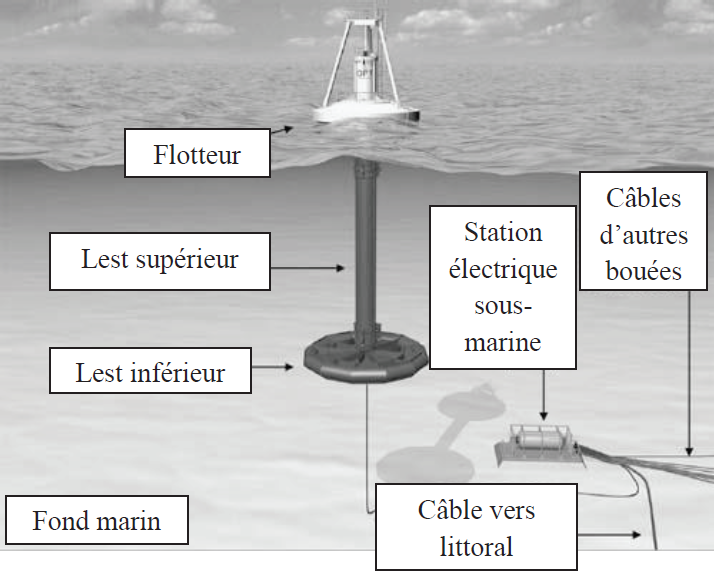
\includegraphics[width=\linewidth]{89_fig_01}
%\textit{}
\end{marginfigure}

Le système de conversion d'énergie est schématisé sur la figue suivante.

Le vérin hydraulique est entraîné par le mouvement relatif de translation entre le flotteur et le lest.
La translation du piston par rapport au cylindre du vérin est donc également paramétrée par le
déplacement $z(t)$ par rapport à la position d’équilibre. La section utile du piston est notée $S_p$. Les
pressions dans les chambres supérieure et inférieure du vérin sont notées respectivement $P_1$ et $P_2$.

Un réservoir accumulateur haute pression (a) et un réservoir accumulateur basse pression (b)
permettent de maintenir les pressions $P_a$ (pression d'admission du moteur hydraulique) et $P_b$
(pression de refoulement du moteur hydraulique) quasi-constantes en régime établi.

Un ensemble de clapets anti-retour permet de générer un débit volumique unidirectionnel $Q_m(t)$
vers le moteur hydraulique, quel que soit le sens de déplacement du piston. Les pertes induites par
ce circuit redresseur seront négligées. On pourra alors considérer en régime établi, et en première
approximation, les relations suivantes entre les pressions dans les réservoirs et dans les chambres du
vérin : $P_a = \text{max} \left(P_1,P_2\right)$ et $P_b = \text{min} \left(P_1,P_2\right)$.

\fi


\question{Compléter les zones en pointillés du schéma hydraulique en dessinant
les clapets anti-retour conformément à la description précédente.}
\ifprof
\begin{corrige}
\begin{center}
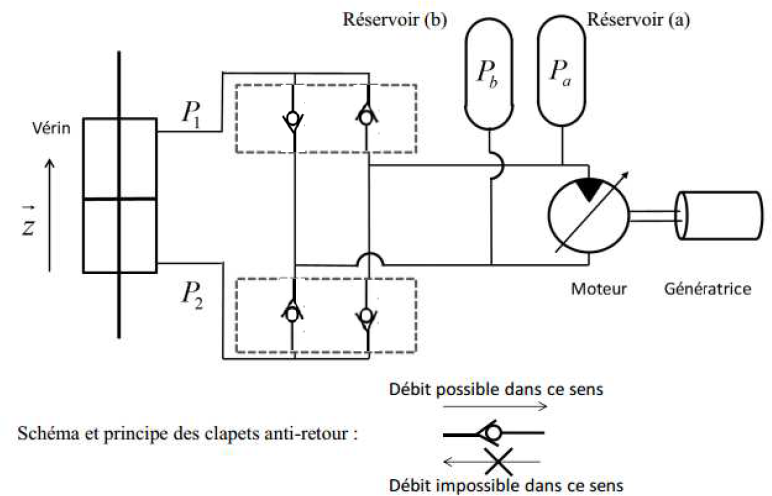
\includegraphics[width=.5\linewidth]{89_cor_01}
%\textit{}
\end{center}
\end{corrige}
\else

\begin{marginfigure}
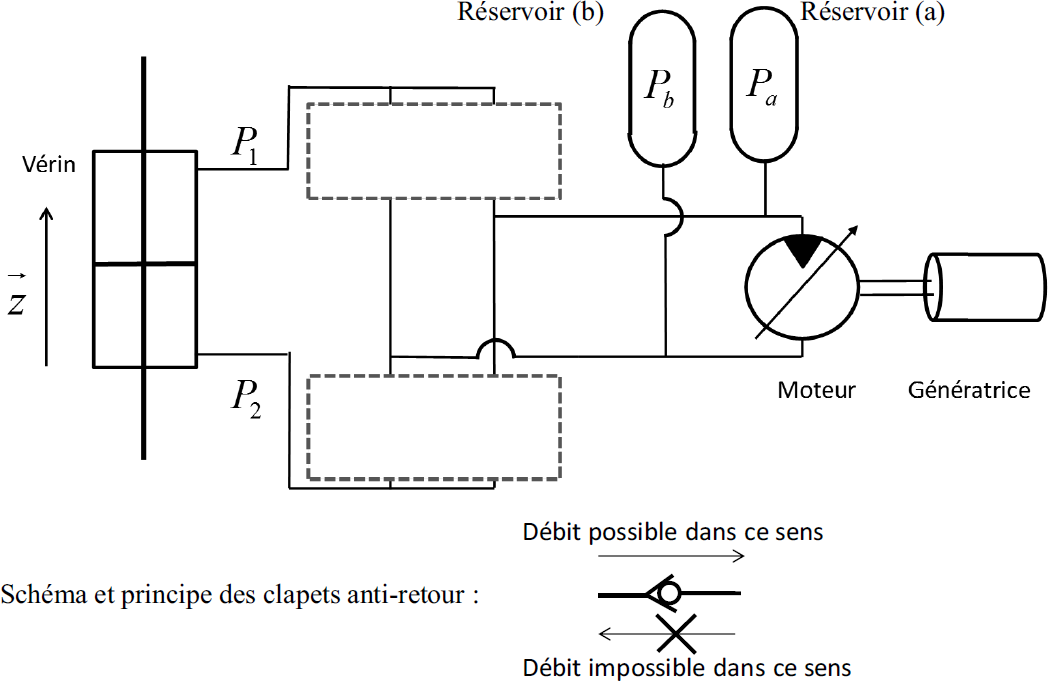
\includegraphics[width=\linewidth]{89_fig_02}
%\textit{}
\end{marginfigure}
\fi

\ifprof
\else
\begin{flushright}
\footnotesize{Corrigé  voir \ref{A3:05:89}.}
\end{flushright}%
\fi 
 
\graphicspath{{\repStyle/png/}{../SYS-01/SYS-01_ChainePuissance/90_Pilote/images/}} 
\normaltrue \difficilefalse \tdifficilefalse
\correctionfalse

%\UPSTIidClasse{11} % 11 sup, 12 spé
%\newcommand{\UPSTIidClasse}{12}
% ATS 2019
\exer{Pilote hydraulique de voilier $\star$ \label{A3:05:90}}
\setcounter{question}{0}
%\UPSTIcompetence[2]{A3-05}
\xpComp{SYS}{01}
\index{Compétence A3-05}
\index{Compétence SYS-01}
\index{Pilote hydraulique}
\index{Caractériser un constituant de la chaîne de puissance}
\index{Distributeur}
\index{Vérin}
\ifcorrection
\else
\marginnote{\textbf{Pas de corrigé pour cet exercice.}}
\fi



\ifprof
\else
On s'intéresse à la distribution d'énergie hydraulique dans le pilote hydraulique de voilier. 

On donne se premier schéma hydraulique. L'énergie est distribuée par un distributeur monostable 2 positions, 2 orifices. 

\begin{marginfigure}
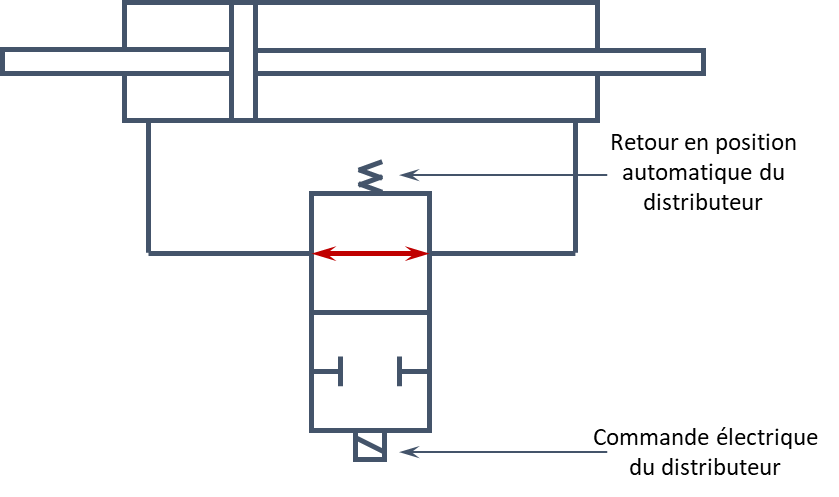
\includegraphics[width=\linewidth]{90_fig_01}
%\textit{}
\end{marginfigure}


\fi


\question{Le schéma précédent est donné dans la situation << au repos >>. Que se passe-t-il si l'utilisateur manipule le vérin à la main ?}
\ifprof
\begin{corrige}
L'huile peut circuler d'une chambre à l'autre en passant par le distributeur. Le vérin peut donc se translater.
\end{corrige}
\else
\fi

\question{On actionne le distributeur. Que se passe-t-il si l'utilisateur manipule le vérin à la main ?}
\ifprof
\begin{corrige}
Le distributeur bloque la circulation de l'huile. Le vérin est bloqué.
%\begin{center}
%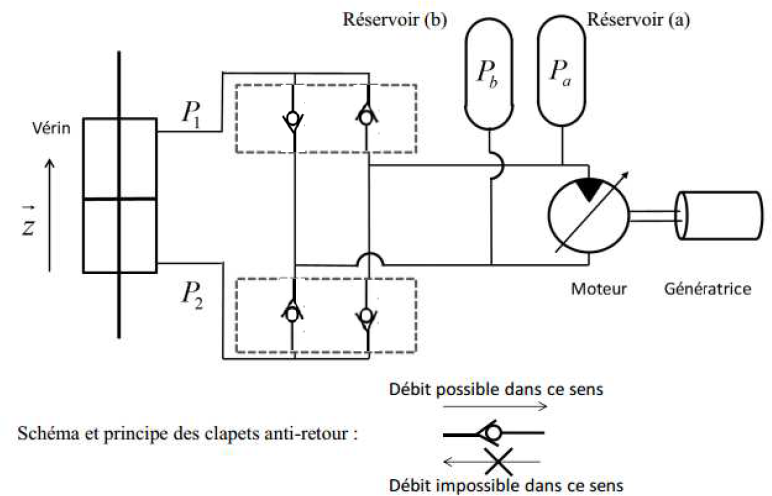
\includegraphics[width=.5\linewidth]{89_cor_01}
%\textit{}
%\end{center}
\end{corrige}
\else
\fi

On complète le schéma avec une motopompe.
\begin{marginfigure}
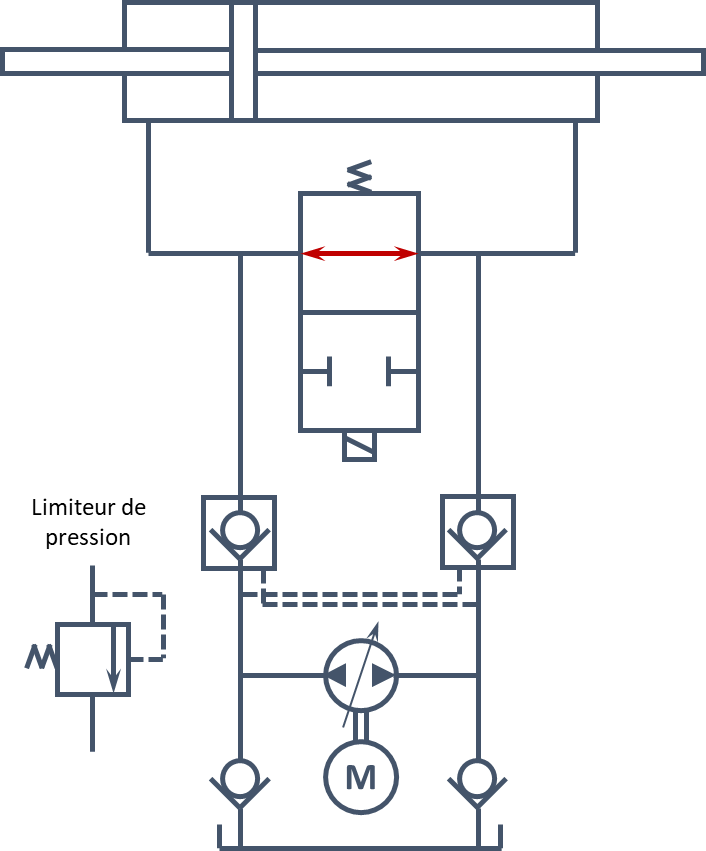
\includegraphics[width=\linewidth]{90_fig_02}
%\textit{}
\end{marginfigure}

\question{On considère le distibuteur activé. Indiquer le sens de fluide permettant de déplacer la tige du vérin vers la gauche. Constatez-vous un problème ?}



\question{Les traits pointillés indiquent un auto-pilotage. Expliquez alors la circulation du fluide ?}


\question{On désire déplacer le vérin vers la gauche, mais la tige est bloquée. Que se passe-t-il ?}

\question{Pour résoudre le problème précédent, on peut utiliser un limiteur de pression. Ajouter le limiteur de pression pour résoudre le problème précédent.}
\ifprof
\else
\begin{flushright}
\footnotesize{Corrigé  voir \ref{A3:05:90}.}
\end{flushright}%
\fi 
 
\section{Analyser une solution technologique} 
\section{Analyser un cahier des charges} 
\section{Valider les performances d'un système vis-à-vis d'un cahier des charges} 
\section{Analyser les résultats d'une simulation ou d'une expérimentation} 
\section{Mesurer et analyser une grandeur physique} 
\setchapterpreamble[u]{\margintoc} 
\chapter{Résoudre un problème de géométrie} 
\section{Analyser la géométrie d'un mécanisme, analyser des surfaces de contact, réaliser des constructions géométriques} 
\section{Modéliser un mécanisme en réalisant un schéma cinématique paramétré} 
\section{Résoudre un problème de géométrie : déterminer la trajectoire d'un point ou déterminer une loi Entrée - Sortie} 
\section{Évaluer expérimentalement des grandeurs géométriques} 
\setchapterpreamble[u]{\margintoc} 
\chapter{Résoudre un problème de cinématique} 
\section{Analyser un mécanisme, réaliser un graphe de liaison} 
\section{Déterminer un vecteur vitesse, un torseur cinématique, un vecteur accélération} 
\section{Déterminer le rapport de transmission d'un transmetteur} 
\section{Déterminer un loi ES cinématique, utiliser l'hypothèse de RSG} 
\section{Évaluer expérimentalement une grandeur cinématique} 
\setchapterpreamble[u]{\margintoc} 
\chapter{Résoudre un problème de statique} 
\section{Analyser un problème en utilisant un graphe de structure} 
\section{Modéliser les actions mécaniques locales, globales, frottement} 
\section{Proposer une démarche de résolution en utilisant le PFS} 
\section{Mettre en œuvre une démarche de résolution} 
\section{Évaluer expérimentalement une action mécanique} 
\setchapterpreamble[u]{\margintoc} 
\chapter{Modéliser un mécanisme} 
\section{Analyser un mécanisme en utilisant un graphe de liaisons} 
\section{Simplifier un mécanisme en utilisant une liaison équivalente} 
\section{Évaluer l'hyperstatisme d'un mécanisme} 
\section{Simplifier un mécanisme pour le rendre isostatique} 
\section{Analyser les conséquences de l'hyperstatisme d'un mécanisme} 
\setchapterpreamble[u]{\margintoc} 
\chapter{Résoudre un problème de dynamique} 
\section{Analyser un problème, définir une loi de mouvement} 
\section{Analyser un mécanisme en utilisant un graphe de structure} 
\section{Modéliser un solide et déterminer ses caractéristiques inertielles} 
\section{Déterminer un torseur cinétique, un torseur dynamique} 
\section{Proposer une démarche de résolution en utilisant le PFD} 
\section{Mettre en œuvre une démarche de résolution en utilisant le PFD} 
\setchapterpreamble[u]{\margintoc} 
\chapter{Résoudre un problème d'énergétique} 
\section{Analyser un mécanisme en utilisant un graphe de structure} 
\section{Déterminer les puissances intérieures} 
\section{Déterminer les puissances extérieures} 
\section{Déterminer l'inertie équivalente, la masse équivalente, l'énergie cinétique, un travail} 
\section{Proposer et mettre en œuvre une démarche de résolution} 
\setchapterpreamble[u]{\margintoc} 
\chapter{Modéliser un SLCI} 
\section{Analyser un asservissement, proposer une structure d'asservissement} 
\section{Modéliser un SLCI en utilisant la transformée de Laplace} 
\section{Modéliser un SLCI en utilisant un schéma-bloc} 
\section{Modéliser un SLCI en utilisant un modèle polyphysique} 
\section{Modéliser un SLCI à plusieurs entrées, sous forme matricielle éventuellement} 
\section{Linéariser un comportement, une équation, simplifier un modèle} 
\section{Modéliser un système d'ordre 1 et d'ordre 2} 
\section{Déterminer une FTBO et une FTBF} 
\section{Identifier des fonctions de transfert (à partir d'un schéma-bloc), mettre sous forme canonique et identifier des constantes} 
\section{Déterminer et identifier une réponse temporelle} 
\section{Déterminer, identifier et analyser une réponse fréquentielle} 
\setchapterpreamble[u]{\margintoc} 
\chapter{Évaluer les performances d'un SLCI} 
\section{Évaluer la stabilité en utilisant la BF, les pôles de la BF} 
\section{Évaluer la stabilité en utilisant les marges de la BO} 
\section{Évaluer la rapidité de la réponse temporelle} 
\section{Évaluer la rapidité à partir de la réponse fréquentielle de la BO} 
\section{Évaluer la précision à partir du TVF} 
\section{Évaluer la précision en utilisant la classe de la BO} 
\setchapterpreamble[u]{\margintoc} 
\chapter{Corriger un SLCI} 
\section{Analyser un choix de correcteur (compensation de pôles, nombre d'intégrations)} 
\section{Régler un correcteur P graphiquement ou analytiquement} 
\section{Régler un correcteur PI graphiquement ou analytiquement} 
\section{Régler un correcteur à avance de phase} 
\section{Modéliser un correcteur numérique} 
\section{Implanter un correcteur sur une cible} 
\setchapterpreamble[u]{\margintoc} 
\chapter{Modélisation des non linéarité d'un système} 
\section{Identifier une non linéarité} 
\section{Modéliser une non linéarité} 
\setchapterpreamble[u]{\margintoc} 
\chapter{Modéliser un système combinatoire ou séquentiel} 
\section{Analyser un système séquentiel en utilisant un chronogramme, analyser un système combinatoire en utilisant une table de vérité} 
\section{Modélisation par équation booléenne} 
\section{Modélisation par diagramme d'état} 
\setchapterpreamble[u]{\margintoc} 
\chapter{Résoudre un problème numériquement} 
\section{Mettre un problème sous forme matricielle} 
\section{Résolution de f(x)=0} 
\section{Résolution d'une équation différentielle} 
\section{Résoudre un problème numériquement} 
\section{Résoudre un problème en utilisant l'apprentissage automatisé} 
